
%%%%%%%%%%%%%%%%%%%%%%%%%%%%%%%%%%%%%%%%%%%%%%%%%%%%%%%%%%%%%%%%%%%%%%%%%%%%%%%
%
%  EGSnrc getting started manual
%  Copyright (C) 2017 National Research Council Canada
%
%  This file is part of EGSnrc.
%
%  EGSnrc is free software: you can redistribute it and/or modify it under
%  the terms of the GNU Affero General Public License as published by the
%  Free Software Foundation, either version 3 of the License, or (at your
%  option) any later version.
%
%  EGSnrc is distributed in the hope that it will be useful, but WITHOUT ANY
%  WARRANTY; without even the implied warranty of MERCHANTABILITY or FITNESS
%  FOR A PARTICULAR PURPOSE.  See the GNU Affero General Public License for
%  more details.
%
%  You should have received a copy of the GNU Affero General Public License
%  along with EGSnrc. If not, see <http://www.gnu.org/licenses/>.
%
%%%%%%%%%%%%%%%%%%%%%%%%%%%%%%%%%%%%%%%%%%%%%%%%%%%%%%%%%%%%%%%%%%%%%%%%%%%%%%%
%
%  Authors:         Reid Townson
%                   Frederic Tessier
%                   Ernesto Mainegra-Hing
%
%  Contributors:
%
%%%%%%%%%%%%%%%%%%%%%%%%%%%%%%%%%%%%%%%%%%%%%%%%%%%%%%%%%%%%%%%%%%%%%%%%%%%%%%%


\documentclass[12pt,twoside]{article}
\setlength{\textwidth}{6.5in}
\setlength{\textheight}{9.3in}
\setlength{\oddsidemargin}{0.0in}
\setlength{\evensidemargin}{0.0in}
\setlength{\topmargin}{-0.6in}
\setlength{\parindent}{1.5em}
\setlength{\topsep}{0ex}
\setlength{\itemsep}{0ex}

\newcommand{\parsp}{~\hspace*{1.5em}}
\setlength{\parskip}{0.1in}
\setlength{\baselineskip}{0.4in}
\newcommand{\head}[1]{\begin{center}\begin{Large}{\bf #1}
                                              \end{Large}\end{center}}
\newcommand{\cen}[1]{\begin{center} #1 \end{center}                   }
\newcommand{\etal}{{\em et.al.}}
\newcommand{\etc}{{\em etc}}
\newcommand{\eg}{{\em e.g.}}
\newcommand{\ie}{{\em i.e.}}

\usepackage{graphicx}
\usepackage{html}
\usepackage{fancyhdr}
\renewcommand{\footrulewidth}{0.4pt}
\renewcommand{\headrulewidth}{0.4pt}

\lhead[{\sffamily \thepage~}]{{\sf NRCC Report PIRS-EGS-101}}
\rhead[{\sf Getting Started with EGSnrc}]{{\sffamily ~\thepage}}
\rfoot{{{\sf \rightmark}}}
\lfoot[{{\sf \leftmark}}]{{\small Last edited $Date: 2017/10/20 09:30:00 $
}}
\cfoot{}

\renewcommand{\refname}{}

% ====================================
% These settings are from EGSnrc labs
\usepackage{fancyvrb}

\usepackage{color}
\definecolor{white}{rgb}{1,1,1}
\definecolor{gray}{rgb}{0.6,0.6,0.6}
\definecolor{red}{rgb}{0.85,0,0}
\definecolor{green}{rgb}{0,0.85,0}
\definecolor{blue}{rgb}{0,0,1}
\definecolor{verb}{cmyk}{1,0.2,0,0.2}
\definecolor{beige}{rgb}{0.92,0.87,0.78}
\definecolor{question}{rgb}{0.1,0.6,0.1}

%% code listings
\usepackage{listings}
\definecolor{terminal}{rgb}{0.91,0.96,0.91}
\definecolor{rule}{rgb}{0.3,0.4,0.3}
\definecolor{prompt}{rgb}{0.6,0.7,0.6}
\definecolor{keyword}{cmyk}{1,0.2,0,0.2}
\definecolor{comment}{rgb}{0.6,0,0}

\lstset{
    language=bash,
    aboveskip=2ex,
    frame=single,
    framerule=0.4pt,
    rulecolor=\color{rule},
    framesep=6pt,
    framexleftmargin=5pt,
    xleftmargin=10pt,
    xrightmargin=5pt,
    framextopmargin=2pt,
    backgroundcolor=\color{terminal},
    basicstyle=\ttfamily,
    breaklines=true,
    postbreak=\mbox{\textcolor{red}{$\hookrightarrow$}\space},
    commentstyle=\color{comment},
    classoffset=0,
    keywordstyle=\color{keyword},
    classoffset=1,
    morekeywords={\$},keywordstyle=\color{prompt},
    classoffset=0
}

\fvset{formatcom=\color{verb}}

% ====================================

\begin{document}

\thispagestyle{empty}

% Make it so lstlisting can be copy/pasted from
\lstset{basicstyle = \ttfamily,columns=fullflexible}

\begin{htmlonly}
For information about the authors and/or institutions involved with this
work, use the links provided in the author list.
\begin{rawhtml}
<br><br>
\end{rawhtml}

\begin{rawhtml}
<br><br>
\end{rawhtml}

\begin{rawhtml}
<br><br>
\end{rawhtml}

Use the Up button to get back to this page from within the document.
\begin{rawhtml}
<BR> <HR> <P>
\end{rawhtml}
\copyright
Copyright 2017, National Research Council of Canada Ottawa
\begin{rawhtml}
<BR> <HR> <P>
\end{rawhtml}
\end{htmlonly}

%\setcounter{page}{1}
\pagestyle{empty}

\title{Getting Started with EGSnrc}
\author{ R. Townson, F. Tessier, E. Mainegra \\
Ionizing Radiation Standards\\
National Research Council of Canada,
Ottawa\\
}

\date{Printed: \today \\
NRCC Report PIRS-EGS-101
\begin{latexonly}
\end{latexonly}
}
\maketitle

\pagenumbering{arabic}
\setlength{\parindent}{0em}

\begin{center}
\begin{Large}
{\bf Abstract}
\end{Large}
\end{center}
This manual is a ``quick start'' guide to help new users get familiar with EGSnrc. A number of complete tutorials are included with general guidance that may be difficult to find in the other manuals. It is suggested that a new user follow along with the document from top to bottom, as the concepts continually build to provide a broad understanding of the capabilities of EGSnrc and the included tools and applications. However, the
information provided here is not complete: please refer to the relevant manuals for full
descriptions.

\newpage
\mbox{}	%blank behind title page
\newpage
\setcounter{page}{1}
\pagestyle{fancy}

\tableofcontents

\newpage

%\pagestyle{myheadings}

\section{What is EGSnrc?}
EGSnrc is a software toolkit to perform Monte Carlo simulation of
ionizing radiation transport through matter. It models the propagation
of photons, electrons and positrons with kinetic energies between
1~keV and 10~GeV, in homogeneous materials. EGSnrc is an
extended and improved version of the Electron Gamma Shower (EGS)
software package originally developed at the Stanford Linear Accelerator
Center (SLAC) in the 1970s. Most notably, it incorporates significant
refinements in charged particle transport, better low energy cross
sections, and the egs++ class library to model elaborate geometries and
particle sources.

EGSnrc is distributed with a wide range of applications (previously referred to
as ``user codes'') that utilize the radiation transport physics to calculate
specific quantities. These codes have been developed by numerous authors over
the lifetime of EGSnrc to support the large user community. For a brief
description of each application, see section \ref{apps}.

\section{Installation}

For the most up-to-date installation instructions, see the wiki section of the
EGSnrc github page:

\href{https://github.com/nrc-cnrc/EGSnrc/wiki/Installation-overview}{https://github.com/nrc-cnrc/EGSnrc/wiki/Installation-overview}

\addtocontents{toc}{\protect\setcounter{tocdepth}{2}}
% From this point on, only show up to \subsection in the ToC

\clearpage
\section{Getting dirty: writing your first EGSnrc application}
\label{myapp}

Before approaching the more formal descriptions, let's dive right in to actually writing a simple application that will utilize the EGSnrc core physics to perform a Monte Carlo simulation. This hands-on approach will hopefully serve as an instructive lesson on what an EGSnrc application really does, how to write input files and perform simulations, and how to decipher the output.

During the installation, two directories were created and assigned to environment variables: \Verb+$HEN_HOUSE+ and \Verb+$EGS_HOME+. To write an application, navigate to \Verb+$EGS_HOME+ using a file browser, or on the terminal.

\subsection{Create a new egs++ application}

Let's create a new egs++ application called \,\Verb|myapp|. All EGSnrc
applications---including the ones you write yourself---must reside in a
folder with the name of the application, within \,\Verb|$EGS_HOME|.
When we say egs++, we are referring to using the c++ class library that was
built to allow for c++ applications to directly interface with
the \,\Verb|MORTRAN3| EGSnrc core.

Start by creating a new directory for your application, \,\Verb|myapp|.
Then copy the following files from the existing application, \,\Verb|tutor7pp|: \,\Verb|array_sizes.h|, \,\Verb|Makefile|.
We will provide the linux commands to do this, using a bash shell
(the first \Verb|$| on the left represents the \textbf{bash} shell command prompt,
so don't type it in):

\begin{lstlisting}
$ cd $EGS_HOME
$ mkdir myapp
$ cd myapp
$ cp ../tutor7pp/array_sizes.h ./
$ cp ../tutor7pp/Makefile ./
\end{lstlisting}

Open the \,\Verb|Makefile| using your text editor of choice, and change
instances of ``tutor7pp'' to ``myapp''. There are only two lines that need
changing; they should now read:

\begin{lstlisting}
USER_CODE = myapp
\end{lstlisting}

and

\begin{lstlisting}
EGSPP_USER_MACROS = myapp.macros
\end{lstlisting}

Create a new file called \,\Verb|myapp.macros|\,, and just save it as an empty
file. This file is just a a placeholder for now - it may be used by
more advanced applications.

Finally, create a new file named \,\Verb|myapp.cpp|\,, and save the following
source code in it:

\begin{lstlisting}[language=c++,backgroundcolor=\color{white}]
#include "egs_advanced_application.h"
APP_MAIN (EGS_AdvancedApplication);
\end{lstlisting}

This is the smallest, fully functional EGSnrc application you can write\,!
You may consider it a bit of a cheat - we are using the defined function macro
\,\Verb|APP_MAIN| to write some code for us.

Compile your application with the \,\Verb|make|\, command, which builds the
executable \,\Verb|myapp|\, and save it under \,\Verb|$EGS_HOME/bin/|. For a
given application, you only need to run \,\Verb|make|\, once
(unless you modify the source code).
\begin{lstlisting}
$ make
\end{lstlisting}

\subsection{Create an egs++ input file}

Next we need to create an input file to define the conditions of the simulation.
Create a new file named \,\Verb|slab.egsinp|\, in the application directory,
\,\Verb|$EGS_HOME/myapp/|\,. Copy and paste the following contents:

\begin{lstlisting}[language=ruby,backgroundcolor=\color{white}]
################################
#
# Simple slab simulation
#
################################


################################
### RUN CONTROL
################################
:start run control:
    ncase = 1e3
:stop run control:


################################
### GEOMETRY
################################
:start geometry definition:

    ### plate
    :start geometry:
        name     = slab
        library  = egs_ndgeometry
        type     = EGS_XYZGeometry
        x-planes = -5, 5            # in cm
        y-planes = -5, 5            # in cm
        z-planes = -10, 0, 0.1, 10  # in cm
        :start media input:
            media = vacuum tantalum
            set medium = 1 1
        :stop media input:
    :stop geometry:

    ### use this geometry for the simulation
    simulation geometry = slab

:stop geometry definition:


################################
### MEDIA
################################
:start media definition:

    ### cutoff energies
    ae  = 0.521
    ap  = 0.010
    ue  = 50.511
    up  = 50

    ### tantalum
    :start tantalum:
        density correction file = tantalum
    :stop tantalum:

    ### lead
    :start lead:
        density correction file = lead
    :stop lead:

    ### water
    :start water:
        density correction file = water_liquid
    :stop water:

:stop media definition:


################################
### SOURCE
################################
:start source definition:

    ### pencil beam
    :start source:
        name      = pencil_beam
        library   = egs_parallel_beam
        charge    = -1
        direction = 0 0 1
        :start spectrum:
            type = monoenergetic
            energy = 20 # in MeV
        :stop spectrum:
        :start shape:
            type     = point
            position = 0 0 -10
        :stop shape:
    :stop source:

    ### use this source for the simulation
    simulation source = pencil_beam

:stop source definition:


################################
### VIEWER CONTROL
################################
:start view control:
    set color = lead      120 120 200 200
    set color = tantalum  120 255 120 255
    set color = water       0 220 255 200
:stop view control:


################################
### AUSGAB OBJECTS
################################
:start ausgab object definition:

    ### particle tracks
    :start ausgab object:
        name    = tracks
        library = egs_track_scoring
    :stop ausgab object:

:stop ausgab object definition:
\end{lstlisting}

We'll get into the meaning of the various input parameters later! For now,
let's just run the simulation and see what happens. The input file models
\textbf{a thousand 20~MeV electrons incident on a 1~mm
thick tantalum plate.}

\begin{lstlisting}
$ myapp -i slab.egsinp
\end{lstlisting}

Here \,\Verb|myapp|\, is the executable name, \,\Verb|-i|\, is a
\textit{flag} to specify the input file \,\Verb|slab.egsinp|. This
simulation runs in less than a second and prints results on the
terminal. It also saves information about the simulated particle tracks
in the file \,\Verb|slab.ptracks|.

Load the \,\Verb|slab.egsinp|\, input file and \,\Verb|slab.ptracks|\, in
\,\Verb|egs_view|\, utility to understand the geometry of the simulation.
Click the \textbf{Show tracks} checkbox, rotate around the scene (left
mouse button in the image window), and zoom in and out (scroll wheel). Pan
the view by holding Ctrl and dragging with the left mouse button.

\begin{lstlisting}
$ egs_view slab.egsinp slab.ptracks
\end{lstlisting}

After turning on particle tracks, \,\Verb|egs_view|\, should display something
like the following image. In the figure, a pencil beam of electrons is impinging
from the left (negative z), towards the right (positive z).
Notice that by hovering your mouse over the plate, you
can investigate the region numbers that were assigned to the geometry. Looking
down a ray from your mouse, the numbers are displayed in the top left. In this
case, the first region the ray sees is the air above the plate (region 0), then
the Ta plate (region 1), then the air below the plate (region 2).

\begin{center}
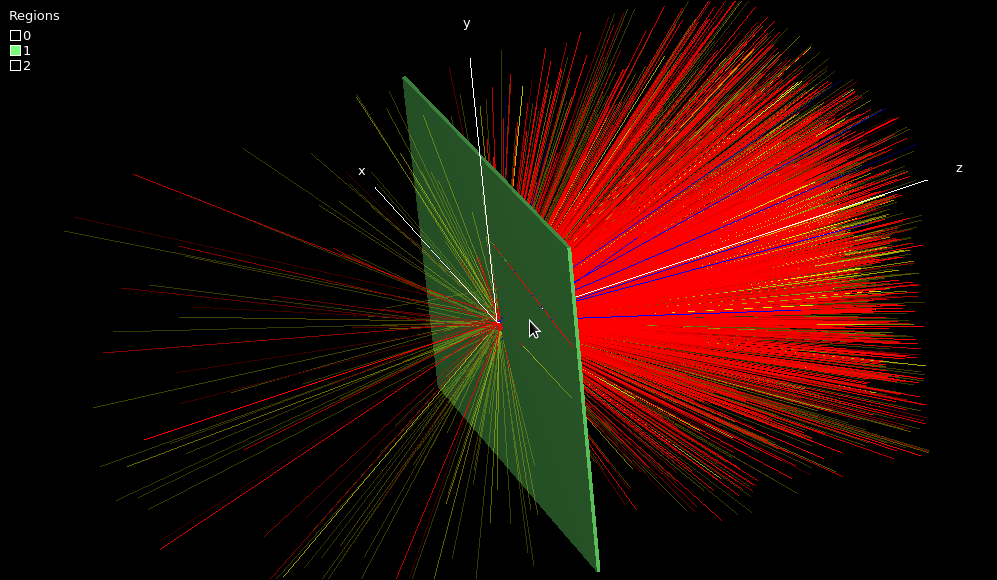
\includegraphics[height=240pt]{figures/ta-plate-example}
\end{center}

Congratulations, you created your first egs++ application and ran
your first simulation\,!

\subsubsection{Question}

\begin{enumerate}
\item Aside from particle tracks, does the \,\Verb|myapp|\, application
provide any useful information when it runs, such as energy deposited,
dose, spectrum, etc.\,?
\end{enumerate}

\clearpage
\subsection{Compile and run using egs\_gui}
All EGSnrc applications can be compiled and run using the GUI, \,\Verb|egs_gui|.
Let's rewind and repeat the \,\Verb|myapp| example using \,\Verb|egs_gui|
instead of the command line.

\begin{enumerate}
\item Open \Verb|egs_gui|, the GUI for compiling and executing any EGSnrc application.
\item Notice that the \Verb|Compile| tab is selected by default. Use the selection box in the bottom left of the GUI, and select \Verb|myapp|.
\item Click the \Verb|Go| button. It will take some time to compile. If you see \Verb|ExitCode = 0| in the output, the application has compiled successfully!
\item Switch to the \Verb|Execute| tab.
\item In the \Verb|PEGS file| section, check the \Verb|pegsless| checkbox.
\item In the \,\Verb|Input file| section, click the \,\Verb|...| button, and
select the input file we created earlier: \,\Verb|slab.egsinp|.
\item To run the simulation, just click \Verb|Start|.
\item The output of the simulation is displayed in the \Verb|egs_gui| output
textbox after executing the simulation. Depending on the application, there
may be additional output in the corresponding application directory in
\Verb|$EGS_HOME|.
\end{enumerate}

\subsection{Add a dose scoring object}

The little application \,\Verb|myapp|\, does not really report any quantity
of interest: by default the egs++ application just transports the
particles in the geometry. It is up to the user to implement methods to
extract information from the simulation.

The easiest way to get results is by adding a dose scoring objects in
your input file. For example, to get a report of the dose deposited in
every region of the geometry at the end of the simulation, \textbf{add}
the following input block \textbf{inside} the existing
\,\Verb|ausgab object definition|\, delimiters at the end of your input
file (you will learn more about the egs++ syntax later). After this, you should
\textbf{only have a single} \,\Verb|ausgab object definition|\,, containing two
\,\Verb|ausgab object|\, blocks.

\begin{lstlisting}[language=ruby,backgroundcolor=\color{white}]
:start ausgab object definition:

    # ... there is an existing object here for ptracks

    :start ausgab object:
        name         = dose
        library      = egs_dose_scoring
        dose regions = 1
        volume       = 10
    :stop ausgab object:

:stop ausgab object definition:
\end{lstlisting}

Run the simulation again, and find the ``Summary of region
dosimetry'' in the output:
\begin{lstlisting}
$ myapp -i slab.egsinp
\end{lstlisting}

\subsubsection{Questions}

\begin{enumerate}

\item How much energy is deposited inside the tantalum plate\,? What is
the dose\,?

\item Can you manually convert the value of deposited energy to dose\,?

\item What is the relative uncertainty on energy and dose, and why is
it the same for both\,?

\item Figure out how to increase the number of electrons by a factor 10
in the input file and run the simulation again. Why has the deposited
energy not increased by a factor 10\,? What happened to the uncertainty\,?

\end{enumerate}


\subsection{Change the type of incident particles}

Figure out how to change the incident particle type to \textit{photons}
instead of electrons in \,\Verb|slab.egsinp|. Save and run the simulation
again for $10^4$ incident photons. Load the particle tracks in
\,\Verb|egs_view|.

\subsubsection{Questions}

\begin{enumerate}
\item Is the simulation faster with electrons or with photons\,?
\item How did the dose change compared to electrons\,?
\item Are positrons generated in this simulation? Is this expected\,?

\end{enumerate}



\subsection{Change the energy of incident particles}

Figure out how to change the incident particle energy to 1~MeV in
\,\Verb|slab.egsinp|. Save and run the simulation again for $10^4$
incident photons. Load the particle tracks in \,\Verb|egs_view|.

\subsubsection{Questions}

\begin{enumerate}
\item What is the biggest qualitative difference with the 20~MeV
scenario\,?
\item Did the dose increase or decrease\,?
\item How about simulation time\,?

\end{enumerate}



\subsection{Change the material of the plate}

Figure out how to change the material of the plate to \,\Verb|lead|\, in
\,\Verb|slab.egsinp|. Use \textbf{100~keV electrons} and run the
simulation again for $10^4$ incident electrons. Load the particle tracks
in \,\Verb|egs_view|. \textit{Hint:} the materials are set in the
\,\Verb|geometry definition|. The \,\Verb|media definition| defines the list of
media that may (or may not) be used by geometries.

\subsubsection{Questions}

\begin{enumerate}
\item What is happening to the electrons hitting the lead plate\,?
\item Is that consistent with the deposited energy\,?
\item What is the file size of \,\Verb|slab.ptracks|\, on disk\,?
\item Run 20~MeV electrons striking a \,\Verb|water|\, plate
and interpret the results. Is deposited energy consistent with the known
stopping power value of \,2.45~MeV~cm$^2$/g\, for 20~MeV
electrons in liquid water\,?

\end{enumerate}

\clearpage
\section{Calculating dose with egs++}
EGSnrc now includes egs++, a C++ class library that interfaces with the EGSnrc core \Verb+MORTRAN3+ code. This allows for applications to be written in C++. In this example, we will execute a simple egs++ application, \Verb+tutor7pp+.

There is an example input file included with \Verb+tutor7pp+, \Verb+test1.egsinp+, found in the application directory (\Verb+$EGS_HOME/tutor7pp+). Let's run \Verb+tutor7pp+ with this example. If you look inside the \Verb+test1.egsinp+ file, the geometry is defined as an infinite slab of tantalum, 1~mm thick. A parallel beam of 20~MeV electrons is directed at the slab, and the simulation runs 1000000 particles. Additionally, \Verb+tutor7pp+ has special scoring options that are not available to other applications (each application may define its own input parameters, though most egs++ inputs are the same). For \Verb+tutor7pp+, the user may define regions in which to score pulse height distributions, and the number of bins in each distribution (this is at the bottom of the input file).

Compile and run \Verb+tutor7pp+ using \Verb+egs_gui+, or on the command line.

If you choose to use the command line, the following commands are an example for linux operating systems:
\begin{lstlisting}
$ cd $EGS_HOME/tutor7pp
$ make clean
$ make
$ tutor7pp -i test1 -p tutor_data | tee test1.output
\end{lstlisting}

Notice that we have modified the execution line above to pipe the output to \Verb+tee+ in order to both display it in the terminal as well as save it in an output file. If you look in the application directory after the simulation, it will contain some new files! Namely:
\begin{lstlisting}[backgroundcolor=\color{white}]
test1.egsdat
test1.output
\end{lstlisting}

The \Verb+.egsdat+ file can generally be ignored - it is used by EGSnrc to restart jobs that crashed, or combine parallel runs. The \Verb+.output+ file is where the output from the simulation was stored (if you ran the simulation using the GUI, this file was not created). Opening the file, we can observe the reflected, deposited and transmitted energy fractions for the simulation of electrons through a single slab. Below this, is the pulse height distribution for region 1 (the slab itself).

\subsection{Write the input file}
The full documentation for egs++ is available online, in PIRS-898:

\href{http://nrc-cnrc.github.io/EGSnrc/doc/pirs898/index.html}{http://nrc-cnrc.github.io/EGSnrc/doc/pirs898/index.html}

All egs++ applications use input files with common input blocks, though each application may add new input blocks or new input parameters. It is strongly recommended to browse the PIRS-898 documentation on common inputs. This will provide an overview of what to expect in an input file.

\href{http://nrc-cnrc.github.io/EGSnrc/doc/pirs898/common.html}{http://nrc-cnrc.github.io/EGSnrc/doc/pirs898/common.html}

To get started writing your first input file:
\begin{itemize}
\item Open your favourite text editor! \textit{On linux, some editor suggestions are kate, gedit, vim, emacs, etc. On windows, perhaps notepad++.}
\item There is not a standard syntax highlighter for \Verb+.egsinp+ files. However, you may want to try highlighting for Ruby - it seems to do a reasonable job of catching the eye.
\item Save a new file with the \Verb+.egsinp+ extension.
\end{itemize}

To get started with egs++ input files, let's work through an example for the \Verb+tutor7pp+ application. Of course, this example will largely translate to any egs++ application, with the exception of the scoring options. If you read through the PIRS-898 documentation on \href{http://nrc-cnrc.github.io/EGSnrc/doc/pirs898/common.html}{common input blocks}, you will recognize that input files contain:

\begin{itemize}
\item Geometries
\item Particle sources
\item Run control
\item MC transport parameters
\item Media (optional)
\item Ausgab output (optional)
\item Scoring options (application specific)
\end{itemize}

\subsubsection{Introduction}
The command line instructions in this tutorial assume you are working on a linux system. Of course, the process is very similar on other operating systems, or using \Verb+egs_gui+.

A simple geometry (water cylinder) is used to showcase the ability to score
dose with the \Verb+egs_dose_scoring+ object. Particle tracks can be generated with
the \Verb+egs_track_scoring+ object. Differences  between isotropic and collimated point
sources are discussed.

This tutorial uses \Verb+tutor7pp+ as the application, so navigate on the command line to the directory
\Verb+$EGS_HOME/tutor7pp+ and build the application using \Verb+make+ if you haven't already:

\begin{lstlisting}
$ cd $EGS_HOME/tutor7pp
$ make clean; make
\end{lstlisting}

\paragraph{Prepare the input file}\mbox{}\\

Start by editing a new file to add all the input blocks necessary to run the
simulation. Note that we will be using the bare minimum, but there are
many more options that can be added. In what follows, step-by-step instructions
are given along with different tasks and questions.

\paragraph{Define a cylindrical water phantom}\mbox{}\\

The first step is to define the geometry, which must be placed between the
\Verb+geometry+ \Verb+definition+ start and stop delimiters in the input file.

First define a cylinder with axis parallel to the $z\!$-axis and 5~cm radius:
\vspace{2ex}
\begin{lstlisting}[language=ruby,backgroundcolor=\color{white}]
:start geometry definition:

  :start geometry:
    library  = egs_cylinders
    type     = EGS_ZCylinders
    name     = the_cylinder
    midpoint = 0 0 0
    radii    = 5
  :stop geometry:

:stop geometry definition:
\end{lstlisting}
\vspace{1ex}

This block defines an \textit{infinitely long} cylinder of 5~cm radius. To
produce a finite cylinder of 10~cm height with its front face at $z=0$, first
define bounding planes and then put everything together using an ND geometry.
Add these geometries to the geometry definition block above.
\vspace{3ex}
\begin{lstlisting}[language=ruby,backgroundcolor=\color{white}]
:start geometry:
    library    = egs_planes
    type       = EGS_Zplanes
    name       = the_planes
    positions  = 0 10
:stop geometry:

:start geometry:
    library    = egs_ndgeometry
    name       = phantom
    dimensions = the_planes the_cylinder
    :start media input:
        media = H2O521ICRU
    :stop media input:
:stop geometry:
\end{lstlisting}
\vspace{1ex}

Notice that we used \Verb+H2O521ICRU+ as a medium. This means that the 521icru PEGS4 data file must be used when running the application.

Don't forget to tell the \Verb+EGS_Application+ which geometry is the simulation
geometry:
\vspace{1ex}

\begin{lstlisting}[language=ruby,backgroundcolor=\color{white}]
simulation geometry = phantom
\end{lstlisting}

After placing all these blocks into the geometry definition block,
visualize the geometry with \Verb+egs_view+ and enjoy the fruit of your hard
work:

\begin{lstlisting}
$ egs_view input_file_name
\end{lstlisting}

There is some description of how to use \Verb+egs_view+ in the \href{http://nrc-cnrc.github.io/EGSnrc/doc/pirs898/group__Geometry.html#geometry_view}{geometry module}.

\subsection{Simulate an isotropic point source}

The next step is defining the source. Similar to the geometry definition block,
you can define as many sources as desired and then choose the one to use for
your simulation.

Define an isotropic point source of 100~keV photons. This source emits particles uniformly in all directions. Position the source at $-100$~cm from the origin on the negative $z\!$-axis:
\vspace{2ex}

\begin{lstlisting}[language=ruby,backgroundcolor=\color{white}]
:start source definition:

   :start source:
      library  = egs_point_source
      name     = the_point_source
      position = 0, 0, -100
      :start spectrum:
          type   = monoenergetic
          energy = 0.1
      :stop spectrum:
      charge = 0
   :stop source:

   simulation source = the_point_source

:stop source definition:
\end{lstlisting}
\vspace{2ex}

\paragraph{Define a dose scoring object}\mbox{}\\

Score dose using the ausgab object \Verb+egs_dose_scoring+ which must be
defined between the \Verb+:start ausgab object definitions:+ delimiter and corresponding \Verb+stop+ delimiter:
\vspace{2ex}

\begin{lstlisting}[language=ruby,backgroundcolor=\color{white}]
:start ausgab object definition:

    :start ausgab object:
        library     = egs_dose_scoring
        volume      = 785.398163397       # in cm^3
        region dose = yes
        name        = my_dose_scoring
    :stop ausgab object:

:stop ausgab object definition:
\end{lstlisting}

where the volume is provided for the cylindrical phantom to be able to compute
the dose. By default volumes are set to 1~cm$\!^3$.

\textbf{Defining number of histories to run}

The last piece of input required for the simulation to run, albeit with many
defaults, is the number of histories to run, \Verb+ncase+. This value is defined in the \Verb+run control+ block

\begin{lstlisting}[backgroundcolor=\color{white}]
:start run control:
    ncase = 100000
:stop run control:
\end{lstlisting}


\paragraph{Run the simulation}\mbox{}\\

To run the simulation type in the following command:

\begin{lstlisting}
$ tutor7pp -i input_file_name -p 521icru
\end{lstlisting}

Since the output goes to the screen by default, you can \textit{pipe} the output to the \Verb+tee+ command to \textit{simultaneously} save the terminal output to a file, for later analysis of the results:
\begin{lstlisting}
$ tutor7pp -i ... -p ... | tee output_file
\end{lstlisting}

\paragraph{Questions}\mbox{}\\

\begin{enumerate}

\item Compare the energy deposited reported
by the \Verb+egs_dose_scoring+ object and the one corresponding to the fraction
of energy deposited reported by \Verb+tutor7pp+. Are they the same\,?
  {\bf Hint:} \Verb+egs_dose_scoring+ uses the source's normalization and
  E$_{\rm tot}$ is the total energy entering the phantom, in MeV.

\item What is the solid angle $\Omega$ subtended by the isotropic source and
the front face of the geometry\,?

\item Compute the efficiency $\varepsilon$ based on the uncertainty in the
energy deposited calculated with the \Verb+egs_dose_scoring+ object
and take note of it for a later comparison with the collimated source.

\end{enumerate}

\subsection{Simulate a collimated source}

Run the same calculation using a collimated source. Add the following source
definition input to the source definition block


{\renewcommand\baselinestretch{1}
\begin{lstlisting}[language=ruby,backgroundcolor=\color{white},language=]
:start source:
    library  = egs_collimated_source
    name     = my_collimated_source
    distance = 100
    :start source shape:
         type     = point
         position = 0 0 -100
    :stop source shape:
    :start target shape:
         library = egs_circle
         radius  = 5
    :stop target shape:
    :start spectrum:
          type   = monoenergetic
          energy = 0.1
    :stop spectrum:
    charge = 0
:stop source:
\end{lstlisting}
}

Set the simulation source to be \Verb+my_collimated_source+. You may want
to make a copy of your input file.

Run the simulation again by issuing the following command (with your choice of names for the input and output files):

\begin{lstlisting}
$ tutor7pp -i myinput -p 521icru | tee myoutput
\end{lstlisting}


\paragraph{Questions}\mbox{}\\

\begin{enumerate}

\item Compare the \textit{fraction} of energy deposited with the result obtained
for the isotropic point source.
Are they the same\,? Explain\,!

\item Compare the energy deposited reported by the \Verb+egs_dose_scoring+
object with the same result obtained earlier for the isotropic point source.
Are they the same\,? Explain\,! \textbf{Hint:} See section \ref{notes} below for a description on how normalization is done in \Verb+EGS_CollimatedSource+.

\item Compute the efficiency based on the uncertainty in the energy deposited
calculated with
the \Verb+egs_dose_scoring+ object
and compare it with the efficiency of the isotropic source. Do you see any
difference\,?

\end{enumerate}


\paragraph{Particles tracks}\mbox{}\\

And now comes the fun part: \textit{particle tracks\,!}

You will be generating particle tracks with the collimated source. To this end,
you must define an \Verb+egs_track_scoring+ object between the
\Verb+ausgab object definition+ delimiters in our input file. Here is an example:
\begin{lstlisting}[language=ruby,backgroundcolor=\color{white}]
:start ausgab object:
    library         = egs_track_scoring
    name            = tracker
    score electrons = no
    score positrons = no
    score photons   = yes
    # start scoring = 0      # default is 0
    # stop  scoring = 1024   # default is 1024
    # buffer size   = 1024   # default is 1024
:stop ausgab object:
\end{lstlisting}

Tracks are only \textit{scored} inside the geometry, hence particle tracks are only generated inside the water cylinder. To see the particle track from the source all the way to the phantom, you need to embed the cylinder and the source inside another geometrical object.

Use a large box of air as an envelope geometry. Add the following two geometries in your geometry definition block:
\begin{lstlisting}[language=ruby,backgroundcolor=\color{white}]
:start geometry:
    library  = egs_box
    box size = 500 500 500
    name     = air_box
    :start media input:
        media = AIR521ICRU
    :stop media input:
:stop geometry:

:start geometry:
   library = egs_genvelope
   name    = phantom_in_air
   base geometry = air_box
   inscribed geometries = phantom
:stop geometry:
\end{lstlisting}

and switch the simulation geometry to be \Verb+phantom_in_air+. Run the
simulation once more with 10 times fewer particles.
This simulation should take a fraction of a second and produce the particle
track file \Verb+myinput.ptracks+. To visualize it launch \Verb+egs_view+ with the name of the tracks file:

\begin{lstlisting}
$ egs_view myinput.egsinp myinput.ptracks
\end{lstlisting}

In the GUI check the box \,\Verb+Show tracks+\, in the Particle Tracks
section to display the tracks. You can also load the track files afterwards as
well with the \textbf{Load tracks} button. To see tracks, make the air box transparent or define a clipping plane. The effect of the collimated source becomes more apparent as one zooms into the picture.

\clearpage
\subsubsection{Notes on collimated point source normalization}
\label{notes}

\Verb+EGS_CollimatedSource+ uses a variance reduction technique that
eliminates the inefficiency of setting particles into motion that may miss the
target. For details see~the appendix in Bielajew, Rogers and Nahum, PMB
\textbf{30}, 419--427, 1985.

Using this approach, one can score a quantity $E$ by adding up
individual contributions $e_i$, and compute the ratio
%
\begin{equation}
\label{per_fluence}
\frac{E}{F} = \frac{\sum\limits_{i=1}^{N_{\Omega}}{w_i'\, e_i}}{(N_{\Omega}/d\,^2)}
\end{equation}
%
to obtain the quantity $E$ per unit fluence $F$, with fluence $F$ defined as
$N_{\Omega}/\Omega/d\,^2$. $N_{\Omega}$ is the number of particles uniformly emitted into
the solid angle $\Omega$ and $w_i'$ accounts for isotropic emission into the target area A.

The ratio per incident history $E/N_{\Omega}$ can be recovered using
\begin{equation}
\label{per_history}
\frac{E}{N_{\Omega}} = \frac{E}{F} \cdot \frac{1}{(\Omega \cdot d\,^2)}\,,
\end{equation}
from where the normalization to number of uniformly emitted particles in 4$\pi$ follows trivially.

\clearpage
\section{Modelling an ionization chamber}
In section \ref{myapp}, we wrote the simplest of egs++ applications and used
\,\Verb|egs_view| for the first time. This geometry viewing tool turns out to be
essential when writing complex geometries - both to visually confirm the
accuracy of the design, and to determine the number assigned to \textit{regions}
in the geometry. In the following sections, use this tool frequently!

The \,\Verb|egs_view| tool actually uses the \,\Verb|HOWFAR|
function of each geometry to render the view. This means that what you see \textit{is
what a particle in your simulation sees}. Note that \,\Verb|egs_view| is only
compatible with egs++ input files (not the \,\Verb|MORTRAN3| codes).

For more explanation of \,\Verb|egs_view|, refer to the online documentation
for the
\href{http://nrc-cnrc.github.io/EGSnrc/doc/pirs898/group__Geometry.html#geometry_view}{geometry module}.

When trying to simulate a particular experiment, constructing the geometry is
half the battle! Take your time to learn what can be done; starting from
a similar example and tweaking it for your purposes is a key time-saver.
There are geometry examples online, and in the distribution:

\,\Verb|$HEN_HOUSE/egs++/geometry/examples|

Before building an ionization chamber, we'll go through a couple
more simple examples. In a text
editor, create a new document with the following geometry input, describing
a cubic box:

{\small
\begin{lstlisting}[language=ruby,backgroundcolor=\color{white}]
:start geometry definition:

    ### a simple box definition
    :start geometry:
        name     = my_box       # this name is up to you
        library  = egs_box
        box size = 10           # length units are cm
        :start media input:
            media = my_medium
        :stop media input:
    :stop geometry:

    ### name of the geometry to load in the viewer
    simulation geometry = my_box

:stop geometry definition:
\end{lstlisting}
}

Note that white space is irrelevant---except for line returns because egs++
reads one input per line. Comment your code as you go, and remember the
\Verb|simulation geometry| input to tell the viewer which geometry to load (by
\textbf{name}).

Media names are up to you: the viewer merely assigns different colors to
different media. These names will ultimately have to be defined in the
\,\Verb|media definition|\, input block to run a simulation. However the viewer
displays media even if they are not yet defined.

For a description of the egs++ input syntax for each geometry, and for input
examples, refer to the online manual:
\Verb|http://nrc-cnrc.github.io/EGSnrc/doc/pirs898/index.html|, in the
\Verb|Geometries| section, e.g., \Verb|Geometries > EGS_Box|.

\vspace{1ex}
\subsection{\label{sec:box}Visualize your geometry with {\tt egs\_view}}

Save your box geometry input in a file named \Verb|simple.egsinp|. From the
directory where you saved the file, launch the geometry viewer:

\begin{lstlisting}
$ egs_view simple.egsinp &
\end{lstlisting}

You should see a red square in the geometry window, along with a \textbf{View
Control} window. The viewer starts with the camera on the positive
z-axis, but you can rotate the geometry in 3D by dragging with the mouse, as
shown in Figure~\ref{fig:box}a.

You can pan the view by dragging while pressing the \Verb|Ctrl| key, and zoom in
and out with the middle mouse button or the mouse wheel. Note that these
manipulations do \textit{not} affect your input: \Verb|egs_view| \textit{never
writes to the input file.}

Spend a few minutes exploring the \textbf{Material colors}, \textbf{View} and
\textbf{Look at} inputs to understand what they control. At any time you can
export the current view as an image with the \textbf{Save image} button, while
the \textbf{Close} button quits the application altogether.

The \textbf{Reload} button reads the input file again, which is useful to update
the view upon modifying the input file, without having to launch the viewer
again. \textit{Be warned however that reloading is not robust: some changes in
the input file may cause the viewer to quit abruptly!}

\subsubsection{Question}
\begin{enumerate}

\item What are the region numbers inside and outside the cube\,?

\end{enumerate}

\vspace{3ex}
\begin{figure}[hb]
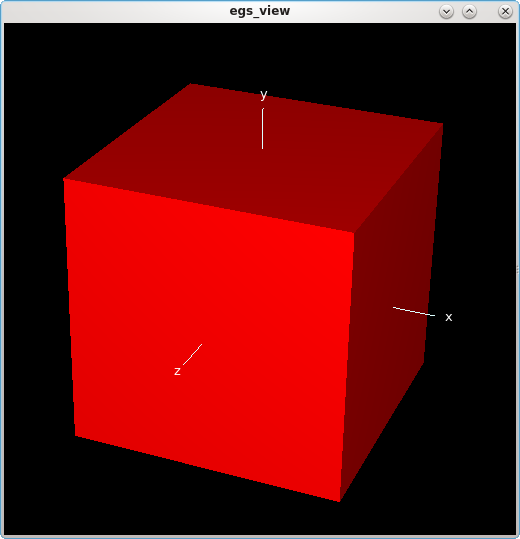
\includegraphics[width=0.49\textwidth]{figures/box}
\hspace{0.02\textwidth}
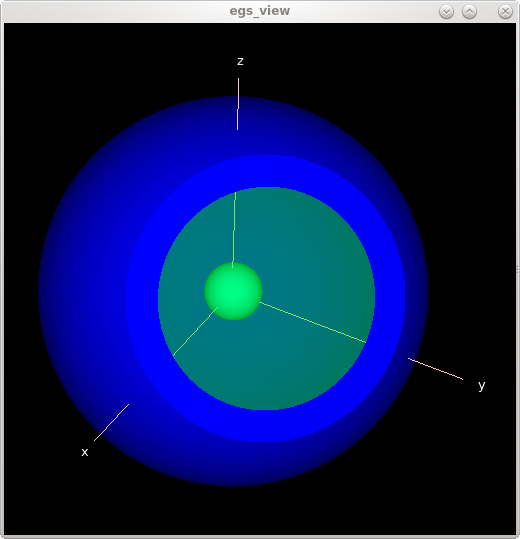
\includegraphics[width=0.49\textwidth]{figures/spheres}
\caption{\label{fig:box} a)~snapshot of the cube defined in the
{\tt simple.egsinp} input file. b)~snapshot of the point of view you
are asked to reproduce using viewer clipping planes in
Section~\ref{sec:clip}.}
\end{figure}


\clearpage
\subsection{\label{sec:clip}Dig in with clipping planes}

Edit your input file to add a second geometry (inside the \textbf{same}
\Verb|geometry definition| input block) defining a set of concentric
spheres:
{\small
\begin{lstlisting}[language=ruby,backgroundcolor=\color{white}]
:start geometry:
    name     = my_spheres   # this name is up to you
    library  = egs_spheres
    radii    = 0.3 1.8 2    # three concentric spheres
    :start media input:
        media = default shell center  # names of media 0 1 2 ...
        set medium = 2 1    # set region 2 to medium 1 (shell)
        set medium = 0 2    # set region 0 to medium 2 (center)
    :stop media input:
:stop geometry:
\end{lstlisting}
}

By default the whole geometry is filled with medium 0 (\Verb|default|, the first
one in the \,\Verb|media|\, list), so it is redundant to specify
\,\Verb|set medium|\, for regions containing medium 0.

Change the \,\Verb|simulation geometry|\, to \,\Verb|my_spheres| (or the name
you
chose) and reload the input in the viewer. You can play with transparency to
reveal the internal structure of the geometry, but clipping planes provide a
more direct route. Click on the \textbf{Clipping planes...} button to access the
planes entry table. Apply a clipping plane oriented along the positive z-axis
and passing through the origin. Make the \Verb|default| medium partially
transparent and rotate the geometry around. Apply a clipping plane to get a view
similar to the one shown in Figure~\ref{fig:box}b.

For clipping planes, \Verb|ax|, \Verb|ay| and \Verb|az| define the unit normal
to a planar surface. The surface can then be offset from the origin by setting
\Verb|d|. \textbf{After typing in the clipping plane, click the ``1''
to select the row}. Then click \textbf{Apply} to update the viewer.
It is possible to use many clipping planes at once! It's a very common
mistake to forget to \textbf{select the clipping plane row} before clicking
\textbf{Apply}.

\subsubsection{Question}

\begin{enumerate}

\item From this point of view, what is the list of regions when you hover your
mouse over the small central sphere\,?

\item What is the region number \textit{outside} the defined geometry\,?

\end{enumerate}


\subsection{Build an egs++ model of the 3C chamber}

Use your newly acquired expertise in egs++ syntax to model the geometry of NRC's
reference ionization chamber "3C", the schematic of which is reproduced in
Figure~\ref{fig:3C}. This is a cylindrically symmetric geometry with 4 distinct
layers along its axis, so the natural option is a \textbf{conestack} geometry.
Put the conestack along the z-axis, and position it according to the numbers
given in the diagram. Below is an input template to get you started. Inspect
the geometry with \Verb|egs_view|.

Read the \href{http://nrc-cnrc.github.io/EGSnrc/doc/pirs898/classEGS__ConeStack.html}{conestack documentation} for more information.

You can expect to end up with 4 layers in the conestack. Since there are no
sloped surfaces (all of the cones are in fact cylinders), the top and bottom
radii will be the same within each layer. Layer 1 requires a single radius,
1.175 for top and bottom. Layer 2 requires two radii for air and graphite,
0.7919 and 1.175, respectively. And so on...

\begin{figure}[ht]
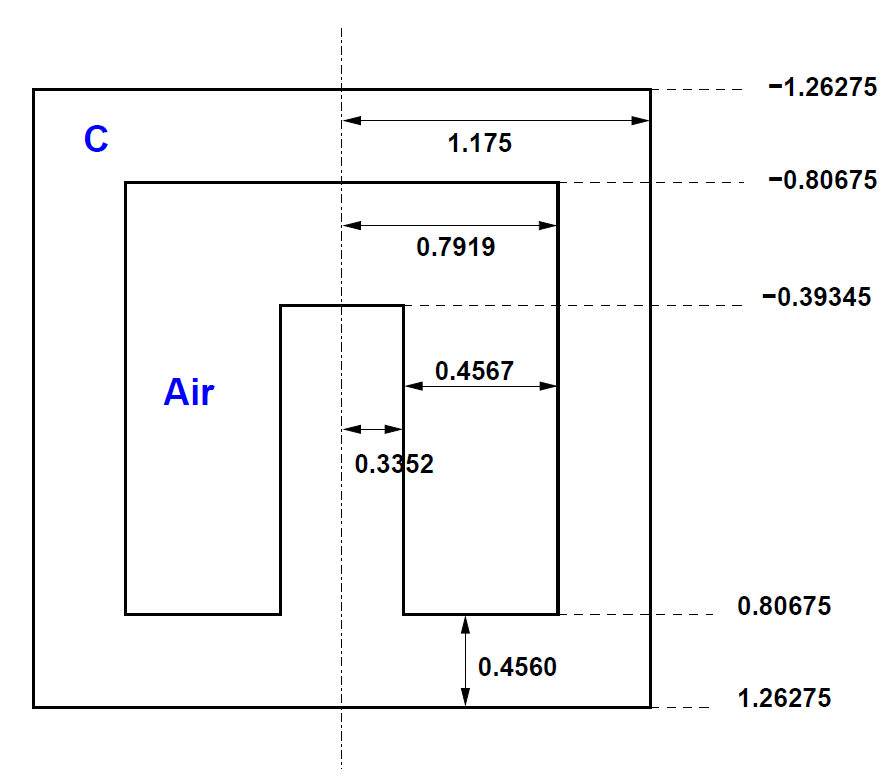
\includegraphics[width=0.7\textwidth]{figures/3C}
\caption{\label{fig:3C} Simplified schematic of NRC's 3C ionization chamber which
is Canada's primary standard for air kerma in a $^{60}$Co beam. Dimensions are in
centimetres. Drawing is not to scale.}
\end{figure}

\vspace{1ex}
{\small
\begin{lstlisting}[language=ruby,backgroundcolor=\color{white}]
:start geometry:
    name    = 3C
    library = egs_cones
    type    = EGS_ConeStack
    axis    = # ... figure out the input for 'axis'

    ### top layer
    :start layer:
        thickness    = # ...
        top radii    = # ...
        bottom radii = # ...
        media        = graphite
    :stop layer:
:stop geometry:
\end{lstlisting}
}

\subsubsection{Questions}

\begin{enumerate}
\item What are the region numbers which correspond to the air cavity\,?
\item Where are regions 1 and 2\,?
\item Can you figure out the conestack region numbering scheme\,?
\end{enumerate}


\subsection{Build an Exradin A12 chamber}
The Exradin A12 is a thimble ionization chamber, shown schematically in
Figure~\ref{fig:a12}. The basic strategy to model such an instrument is to use a
conestack for most of the chamber, which is cylindrically symmetric, except for
the spherical tip. Build the chamber tip with \textbf{spheres} (as shown by
dashed lines in the diagram) and join it with the 7-layer \textbf{conestack}
chamber body, using a composite \textbf{cd geometry}.

\begin{figure}[h]
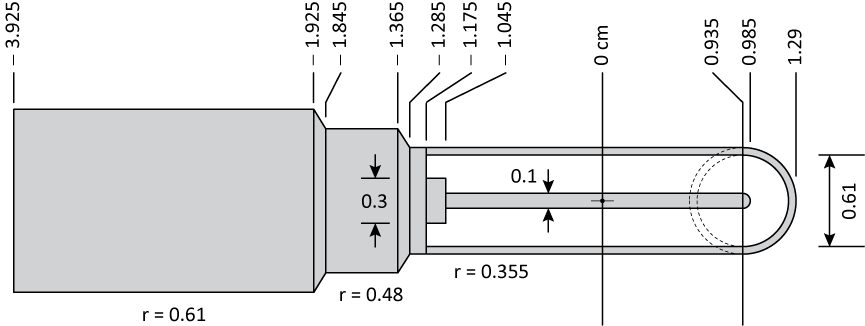
\includegraphics[width=\textwidth]{figures/a12}
\caption{\label{fig:a12}Simplified schematic of an Exradin A12 thimble chamber,
based on information from the manufacturer's product brochure. All units are in
centimetres. Radial dimensions are given, as well as the position of the various
points along the chamber's axis (with the centroid of the collecting volume at
0~cm). The central electrode, the thimble shell and the chamber body are made of
C552 plastic.} \end{figure}

\subsubsection{Model the spherical chamber tip}

Start a new input file for this chamber geometry. Save this input file in
the \,\Verb|$EGS_HOME/egs_chamber| directory. It is recommended to use the
\,\Verb|egs_chamber| application for ionization chamber simulations due to
its useful suite of variance reduction parameters. There are a number of
useful features, found in the \href{http://nrc-cnrc.github.io/EGSnrc/doc/pirs898/egs_chamber.html}{egs\_chamber documentation}.

Define a geometry for the
chamber tip using \textbf{3 concentric spheres,} as in Section~\ref{sec:clip}.
The smallest sphere will become the spherical tip of the central electrode\,!
Position the midpoint of the set of spheres on axis in their final location at
$x=0.935$~cm, as shown in Figure~\ref{fig:a12}.

\textbf{Include the following} bounding
box view control input block in your input file (\textit{outside} the geometry
definition block) to help the viewer find the spheres. Inspect the geometry in
\Verb|egs_view|.

{\small
\begin{lstlisting}[language=ruby,backgroundcolor=\color{white}]
:start view control:
    xmin = -4
    xmax =  4
    ymin = -4
    ymax =  4
    zmin = -4
    zmax =  4
:stop view control:
\end{lstlisting}
}

\subsubsection{Model the chamber body}

Use a \textbf{conestack} to define the cylindrically symmetric chamber body. In
the next step you will join this conestack to the spheres using a cd geometry
plane located at $x=0.935$~cm.

%Note that when the \Verb|top radii| in a conestack layer are the same as the
%\Verb|bottom radii| of the \textit{previous} layer, it is more efficient to
%omit the \Verb|top radii| input, \eg,

%{\small
%\begin{lstlisting}[backgroundcolor=\color{white}]
%:start layer:
%    thickness   = 1
%    top radii    = 0.05 0.355
%    bottom radii = 0.05 0.355
%:stop layer:
%
%:start layer:
%    thickness   = 0.5
%    # omitted the top radii input: assumed equal to 0.05 0.355
%    bottom radii = 0.08 0.61
%:stop layer:
%\end{lstlisting}
%}

\subsubsection{Join the chamber body to the chamber tip}

Create a set of \textbf{3 planes} perpendicular to the chamber axis, so as to
define two regions, numbered 0 and 1. The middle plane should be located at the
joining point $x=0.935$~cm. The other two planes should be located beyond the
chamber on either side.

{\small
\begin{lstlisting}[language=ruby,backgroundcolor=\color{white}]
:start geometry:
    name      = cd_planes
    library   = egs_planes
    type      = EGS_Xplanes
    positions = # ...
:stop geometry:
\end{lstlisting}
}

Finally, use a \textbf{cd geometry} to combine the chamber body and the chamber
tip, using the planes you just defined as the base geometry. Put the body in
region 0, and the tip spheres in region 1. Verify your geometry visually in
\Verb|egs_view|. The cd geometry package is very useful for combining and
cutting geometries. Check out the
\href{http://nrc-cnrc.github.io/EGSnrc/doc/pirs898/classEGS__CDGeometry.html#details}{relevant documentation}
for more information.

{\small
\begin{lstlisting}[language=ruby,backgroundcolor=\color{white}]
:start geometry:
    name    = chamber
    library = egs_cdgeometry
    base geometry = cd_planes
    set geometry  = 0 chamber_body
    set geometry  = 1 chamber_tip
:stop geometry:
\end{lstlisting}
}

It is important to avoid having surfaces perfectly abutting (touching)
in egs++, so start your cone\-stack at a location $x>0.935$~cm to avoid touching
the conestack surface to the egs\_planes geometry. To do this, make the top layer
slightly thicker (say 0.05~cm thicker, making it
$1.045+.935+.05=2.03$~cm), and position the conestack at
$0.935+0.05=0.985$~cm to effectively bleed the conestack into the other
geometry. The cd geometry will cut this extra bit off at the plane we define,
giving priority to the chamber tip.

\begin{center}
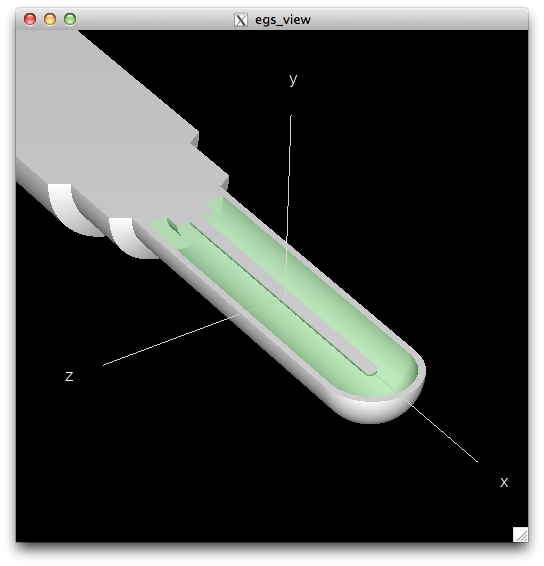
\includegraphics[height=240pt]{figures/a12view}
\end{center}

\subsubsection{Questions}

\begin{enumerate}

\item What are the region numbers that correspond to the air cavity\,?

\item Why is the region for the spherical tip of the air cavity so large\,?

\item How many regions are there in total in this model\,? How
many \textit{real} regions\,?

\item What is the largest region number in this geometry\,?

\end{enumerate}

\subsubsection{Add a region label for the cavity}
You have already determined the region numbers for the cavity, but what happens
if you add more components to the geometry? The global region number might
change! For example, if we inscribe the chamber in a box of water and look
at the region numbers of the cavity again, they may be different. If you need
to know the cavity region numbers for scoring quantities (we will), this can
be quite inconvenient. Instead, use region labels. This assigns a series
of local regions within a given geometry to a label that you can reference
elsewhere.

Local region numbers are what you find when viewing a particular geometry
(e.g. our geometry by the name of \,\Verb|chamber|). To find the local
region numbers just set that geometry as the calculation geometry, and
open \,\Verb|egs_view|. In contrast, the global region numbers are the
numbers that get assigned to those same regions when you load your
\textit{actual} calculation geometry (for example, your chamber inscribed in
water).

To add a region label, place the following \textit{within a geometry block}.
In this example we give the label the name \,\Verb|myLabel|
(make sure it's unique!) and assigned the local regions 0, and 2.
Now if we want to reference those regions later on (in the scoring options),
we can reference the label instead of the global region numbers (which may
change).

{\small
\begin{lstlisting}[language=ruby,backgroundcolor=\color{white}]
set label = myLabel 0 2 55
\end{lstlisting}
}

For example:

{\small
\begin{lstlisting}[language=ruby,backgroundcolor=\color{white}]
:start geometry:
    name    = chamber
    library = egs_cdgeometry
    base geometry = cd_planes
    set geometry  = 0 chamber_body
    set geometry  = 1 chamber_tip

    # The label for the cavity regions
    # View the chamber geometry alone to find these numbers
    set label = chamber_cavity_label 4 1 22
:stop geometry:
\end{lstlisting}
}

\subsubsection{Add a particle source}
For now we will add a simple collimated source. To model a linear accelerator,
you may need to replace this with a \href{http://nrc-cnrc.github.io/EGSnrc/doc/pirs898/classEGS__BeamSource.html}{BEAMnrc shared library source}, or a \href{http://nrc-cnrc.github.io/EGSnrc/doc/pirs898/classEGS__PhspSource.html}{phase-space source}.

{\small
\begin{lstlisting}[language=ruby,backgroundcolor=\color{white}]
:start source definition:

    :start source:
        name    = photons
        library = egs_collimated_source
        charge  = 0
        :start source shape:
            type = point
            position = 0 0 -100
        :stop source shape:
        :start target shape:
            library = egs_rectangle
            rectangle = -5 -5 5 5
        :stop target shape:
        :start spectrum:
            type = monoenergetic
            energy = 10
        :stop spectrum:
    :stop source:

    simulation source = photons

:stop source definition:
\end{lstlisting}
}

\subsubsection{Add transport parameters}
For ionization chamber simulation, it is OK to use most of the EGSnrc default
settings. It is recommended to use \,\Verb|ECUT=0.521| and \,\Verb|PCUT=0.01|.

{\small
\begin{lstlisting}[language=ruby,backgroundcolor=\color{white}]
:start MC transport parameter:

    Global Ecut                 = 0.521
    Global Pcut                 = 0.01
    Rayleigh scattering         = On
    Brems cross sections        = NRC
    Brems angular sampling      = KM

:stop MC transport parameter:
\end{lstlisting}
}

\subsubsection{Add variance reduction}
These variance reduction parameters are valid \textit{only for egs\_chamber}.
They are designed specifically for high efficiency in ionization chamber
simulations.

{\small
\begin{lstlisting}[language=ruby,backgroundcolor=\color{white}]
:start variance reduction:

    cs enhancement  = 1             # use cross-section enhancement

    :start range rejection:
        rejection       = 128
        Esave           = 0.521     # 0.521 implies no range rejection
        cavity geometry = cavity    # this is just a dummy
        rejection range medium = water
    :stop range rejection:

:stop variance reduction:
\end{lstlisting}
}



\clearpage
\section{EGSnrc overview: the applications}
\label{apps}

\addtocontents{toc}{\protect\setcounter{tocdepth}{3}}
% From this point on, only show up to \subsubsection in the ToC

\begin{itemize}
\item EGSnrc is a collection of generic routines that simulate the transport
and interactions of photons, electrons and positrons in matter.
\item The majority of users do not write their own applications - the codes distributed
with EGSnrc are useful for a wide range of calculations.
\item Users can write their own applications that take advantage of the EGSnrc
system, or \textit{toolkit}, by writing a program which specifies their
particular problem in the \Verb+MAIN+ program and communicates with EGSnrc
through the user-supplied routines \Verb+AUSGAB+, \Verb+HOWFAR+ and \Verb+HOWNEAR+
and the EGSnrc routines \Verb+HATCH+ and \Verb+SHOWER+.
\item In principle, applications can be written in any programming language as
long as it can interface with the Fortran EGSnrc code-base.
\item Most commonly, applications are written in \Verb+MORTRAN3+ (native EGSnrc
language) or C++, although they could also be written in \Verb+FORTRAN+ or C.
\end{itemize}

\begin{center}
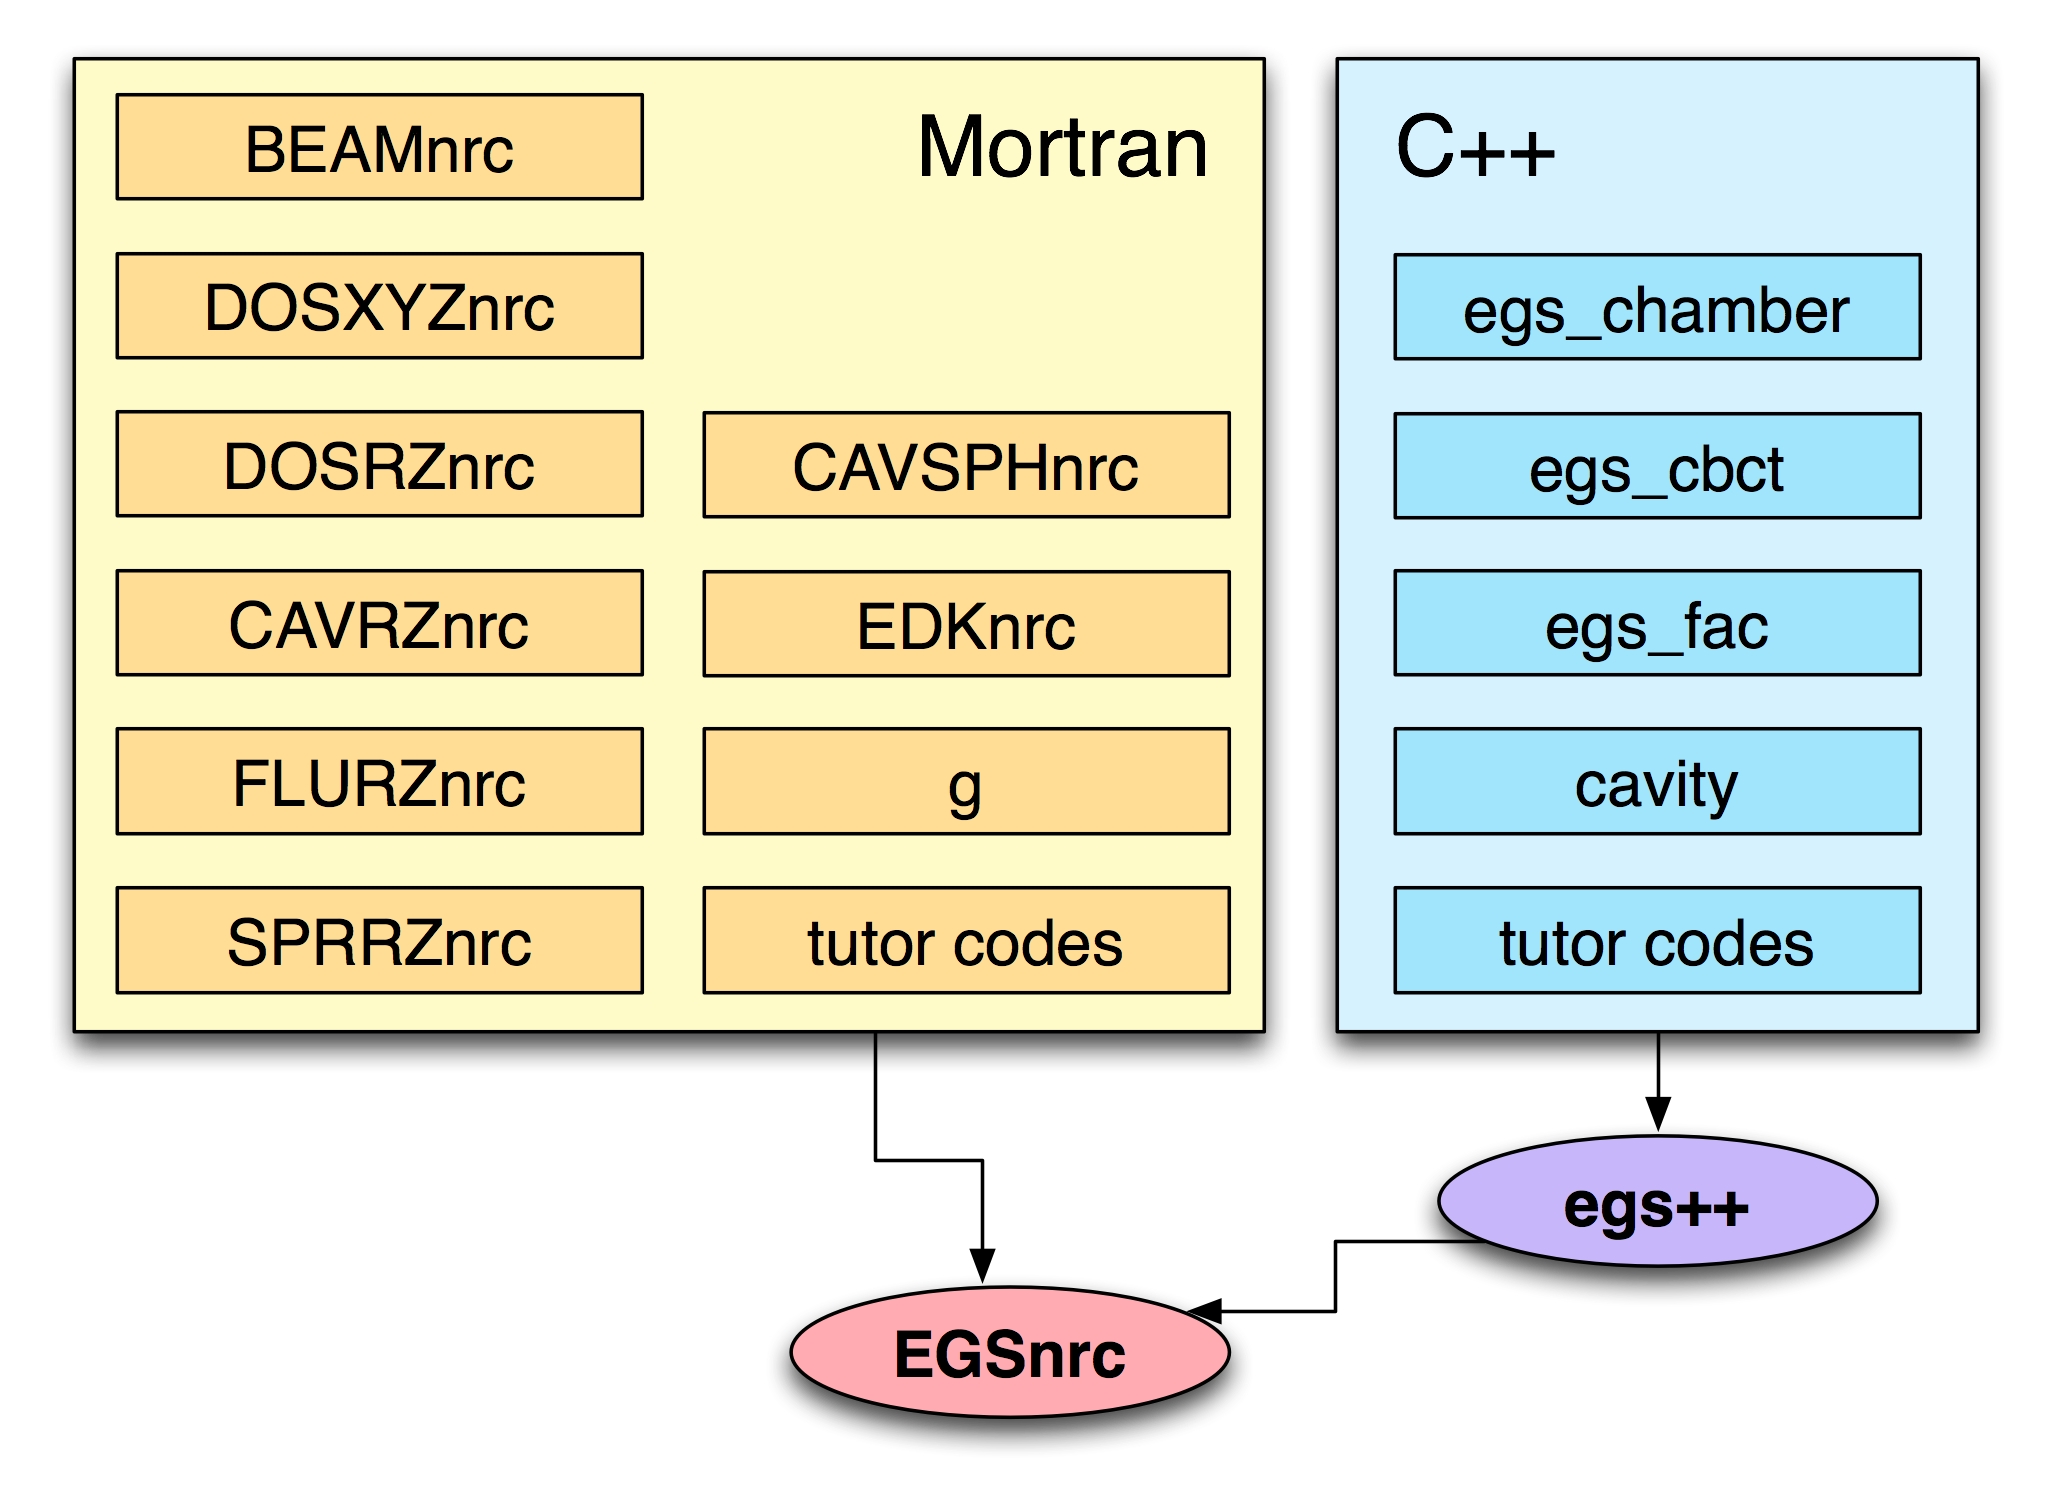
\includegraphics[height=340pt]{figures/egsApplications}
\end{center}

EGSnrc source code: \Verb+$HEN_HOUSE/src/egsnrc.mortran+

EGSnrc global variables: \Verb+$HEN_HOUSE/src/egsnrc.macros+

GUI: \Verb+~/EGSnrc/HEN_HOUSE/gui/egs_gui+

\subsection{BEAMnrc}
\begin{itemize}
\item Ideal for linear accelerator modelling and x-ray systems
\item Includes geometries (called component modules) that can easily represent flattening filters, collimators, MLCs, etc.
\item Accelerators can be compiled as shared libraries to be used as a particle source for other applications
\item Includes time-synchronized capabilities (e.g. dynamic jaws and MLCs)
\item Written in MORTRAN3
\end{itemize}

Documentation: \href{http://nrc-cnrc.github.io/EGSnrc/doc/pirs509a-beamnrc.pdf}{PIRS-509a}

Source code: \Verb+$HEN_HOUSE/omega/beamnrc+

Global variables: \Verb+$HEN_HOUSE/omega/beamnrc/beamnrc_user_macros.mortran+

GUI (launch with \Verb+wish+): \Verb+$HEN_HOUSE/omega/progs/gui/beamnrc/beamnrc_gui.tcl+

\subsection{DOSXYZnrc}
\begin{itemize}
\item Performs dose calculations in voxelized phantoms
\item Includes a variety of source models (e.g. a BEAMnrc shared library)
\item Includes time-synchronized capabilities
\item Written in MORTRAN3
\end{itemize}

Documentation: \href{http://nrc-cnrc.github.io/EGSnrc/doc/pirs794-dosxyznrc.pdf}{PIRS-794}

Source code: \Verb+$HEN_HOUSE/user_codes/dosxyznrc+

Global variables: \Verb+$HEN_HOUSE/user_codes/dosxyznrc/dosxyznrc_user_macros.mortran+

GUI (launch with \Verb+wish+): \Verb+$HEN_HOUSE/omega/progs/gui/dosxyznrc/dosxyznrc_gui.tcl+

\subsection{The RZ applications (cylindrical symmetry)}
These applications are based on cylindrically symmetric geometries and are
written in \Verb+MORTRAN3+. There is a dedicated GUI to compile these
applications and write / edit input files.

Documentation: \href{http://nrc-cnrc.github.io/EGSnrc/doc/pirs702-egsnrc-codes.pdf}{PIRS-702}

GUI documentation: \href{http://nrc-cnrc.github.io/EGSnrc/doc/pirs801-egsinprz.pdf}{PIRS-801}

Source code: \Verb+$HEN_HOUSE/user_codes+

GUI: \Verb+$HEN_HOUSE/gui/egs_inprz+

\subsubsection{DOSRZnrc}
\begin{itemize}
\item Dose and kerma calculations
\end{itemize}
\subsubsection{CAVRZnrc}
\begin{itemize}
\item Calculates ionization chamber correction factors and relevant quantities
\end{itemize}
\subsubsection{FLURZnrc}
\begin{itemize}
\item Particle fluence calculations
\end{itemize}
\subsubsection{SPRRZnrc}
\begin{itemize}
\item Calculates Spencer-Attix spectrum averaged stopping-power ratios for arbitrary media
\end{itemize}

\subsection{The SPH applications (spherical symmetry)}
These applications are based on spherically symmetric geometries and are
written in the fortran preprocessor language \,\Verb|MORTRAN3|.

Documentation: \href{http://nrc-cnrc.github.io/EGSnrc/doc/pirs702-egsnrc-codes.pdf}{PIRS-702}

Source code: \Verb+$HEN_HOUSE/user_codes+

\subsubsection{CAVSPHnrc}
\begin{itemize}
\item Identical to CAVRZnrc but for spherical geometries
\end{itemize}
\subsubsection{EDKnrc}
\begin{itemize}
\item Calculates energy deposition kernels for photons or electrons forced to interact
at the centre of a spherical phantom
\item Also calculates dose distributions in the entire phantom or the dose to specific regions defined as the cavity of a spherical ion chamber
\end{itemize}

\subsection{g}
\begin{itemize}
\item Calculates the energy fraction lost to radiation when electrons slow down (if the incident beam is photons), or the radiative yield (if the incident beam is electrons)
\item Calculates quantities such as mu\_tr, mu\_en and g-bar (the average fraction of energy lost to radiation needed for the calculation of mu\_en)
\item Written in \Verb+MORTRAN3+
\end{itemize}

Source code: \Verb+$HEN_HOUSE/user_codes/g+

\subsection{egs\_chamber}
\begin{itemize}
\item Calculates dose and energy deposited in regions/media
\item Optimized for ionization chamber calculations
\item Many relevant variance reduction techniques
\item Written in c++ (egs++ application)
\end{itemize}

Documentation: \href{http://nrc-cnrc.github.io/EGSnrc/doc/pirs898/egs\_chamber.html}{PIRS-898/egs\_chamber}

Source code: \Verb+$HEN_HOUSE/user_codes/egs_chamber+

\subsection{egs\_cbct}
\begin{itemize}
\item Main goal is the fast estimation of the scatter contribution to an ideal detector in a cone-beam CT (CBCT) setup by means of sophisticated variance reduction techniques and a smoothing algorithm
\item Can also be used for estimating the total signal to the detector and its individual components: transmitted and scattered
\item Initially designed for the purpose of simulating a CBCT setup, but can be equally used for modelling conventional CT scanner setups
\item Written in c++ (egs++ application)
\end{itemize}

Documentation: \href{http://nrc-cnrc.github.io/EGSnrc/doc/pirs898/egs\_cbct.html}{PIRS-898/egs\_cbct}

Source code: \Verb+$HEN_HOUSE/user_codes/egs_cbct+

\subsection{egs\_fac}
\begin{itemize}
\item Designed for the purpose of calculating free air chamber (FAC) correction factors
\item Written in c++ (egs++ application)
\end{itemize}

Documentation: \href{http://nrc-cnrc.github.io/EGSnrc/doc/pirs898/egs\_fac.html}{PIRS-898/egs\_fac}

Source code: \Verb+$HEN_HOUSE/user_codes/egs_fac+

\subsection{cavity}
\begin{itemize}
\item Calculates dose in ionization chamber and correction factors
\item The predecessor of egs\_chamber and egs\_fac
\item Written in c++ (egs++ application)
\end{itemize}

Documentation: \href{http://nrc-cnrc.github.io/EGSnrc/doc/pirs898/cavity.html}{PIRS-898/cavity}

Source code: \Verb+$HEN_HOUSE/user_codes/cavity+

\subsection{Tutorials (the tutor codes)}
\begin{itemize}
\item Many tutorial applications are distributed, written both in \Verb+MORTRAN3+ and c++
\item The codes are heavily documented and intended to teach the user how to write EGSnrc applications
\end{itemize}

Source code: \Verb+$HEN_HOUSE/user_codes+

\clearpage
\section{Online resources}

\subsection{EGSnrc on github}

\begin{itemize}
\item EGSnrc can be downloaded (or ``cloned'') from the \Verb+github+ page. Make sure
to read the \href{https://github.com/nrc-cnrc/EGSnrc/wiki/Installation-overview}{installation instructions} carefully!

\href{https://github.com/nrc-cnrc/EGSnrc}{https://github.com/nrc-cnrc/EGSnrc}

\item The annual releases can be found on the github release page. Additionally,
pre-compiled GUIs, manuals and sample data are available:

\href{https://github.com/nrc-cnrc/EGSnrc/releases}{https://github.com/nrc-cnrc/EGSnrc/releases}

\item See the \Verb+wiki+ page for release notes, technical instructions and links to online documentation:

\href{https://github.com/nrc-cnrc/EGSnrc/wiki}{https://github.com/nrc-cnrc/EGSnrc/wiki}
\end{itemize}

\subsection{Bug reports}
Have you found a bug? Report it on the github \Verb+issues+ page! Make sure to include sufficient information for us to reproduce the bug.

\href{https://github.com/nrc-cnrc/EGSnrc/issues}{https://github.com/nrc-cnrc/EGSnrc/issues}

\subsection{Submitting your code}
Have you added a feature or fixed a bug? Submit the changes as a \Verb+pull request+! This requires learning the basics of ``git'' - if that is not feasible, you can also submit the changes as an \Verb+issue+ and allow one of us to create the pull request.

\href{https://github.com/nrc-cnrc/EGSnrc/pulls}{https://github.com/nrc-cnrc/EGSnrc/pulls}

\subsection{How to get support}
If you have a question, or encounter problems while using EGSnrc, seek support on the EGSnrc google+ community! This is the best place to get answers to questions ranging from very simple to quite complex. There are 800+ members who regularly answer questions, and the EGSnrc developers also contribute frequently.

\href{https://plus.google.com/communities/106437507294474212197}{https://plus.google.com/communities/106437507294474212197}

To increase your chances of getting an answer, make sure to include as much information as possible in your original post. This should include:
\begin{itemize}
\item The EGSnrc application and version
\item Operating system
\item A clear description of the problem
\item Copy/pasted output including any errors
\item Optionally: screenshots, input files and figures
\end{itemize}

\subsection{Documentation}
Documentation for EGSnrc is available online! However, keep in mind
that the documentation applies to the most recent \Verb+release+ of EGSnrc.
In other words, the documentation is generated annually, at the same time as the
release of the master branch (usually in January).

The online documentation:

\href{http://nrc-cnrc.github.io/EGSnrc/}{http://nrc-cnrc.github.io/EGSnrc/}

If you are using an older version of EGSnrc, or if you are working on the
\Verb+develop+ experimental branch, there may be some differences in the documentation. To obtain the documentation that exactly matches your installation, find the documentation source code within your installation:

\Verb+$HEN_HOUSE/docs/src+

Some additional steps are required to compile the documentation locally.

\subsubsection{Compiling documentation locally}
\begin{enumerate}
\item Install a \latex suite that includes \Verb+pdflatex+, \Verb+bibtex+, \Verb+texmf+ and \Verb+makeindex+ (e.g. \Verb+texlive+)
\item Install \Verb+doxygen+
\item \Verb+cd $HEN_HOUSE/docs/src+ (linux instructions)
\item \Verb+./makedoc.sh all+ (linux instructions)
\end{enumerate}

\clearpage
\section{EGSnrc file structure}
\begin{itemize}
\item \Verb+$HEN_HOUSE+: Points to location of the EGSnrc system (\textbf{user-defined})

\item \Verb+$EGS_HOME+: Points to user's working directory, where applications are copied (\textbf{user-defined})
\end{itemize}

\textbf{BEWARE:} Path to these folders cannot have spaces! EGSnrc relies on GNU \Verb+make+ which doesn't handle blank spaces in names. Also avoid special characters like $\&$.

\subsection{The \$HEN\_HOUSE}
The \Verb+$HEN_HOUSE+ directory contains all source code and data files for the
EGSnrc system. After installation, the contents of this directory generally remain unchanged.
\begin{center}
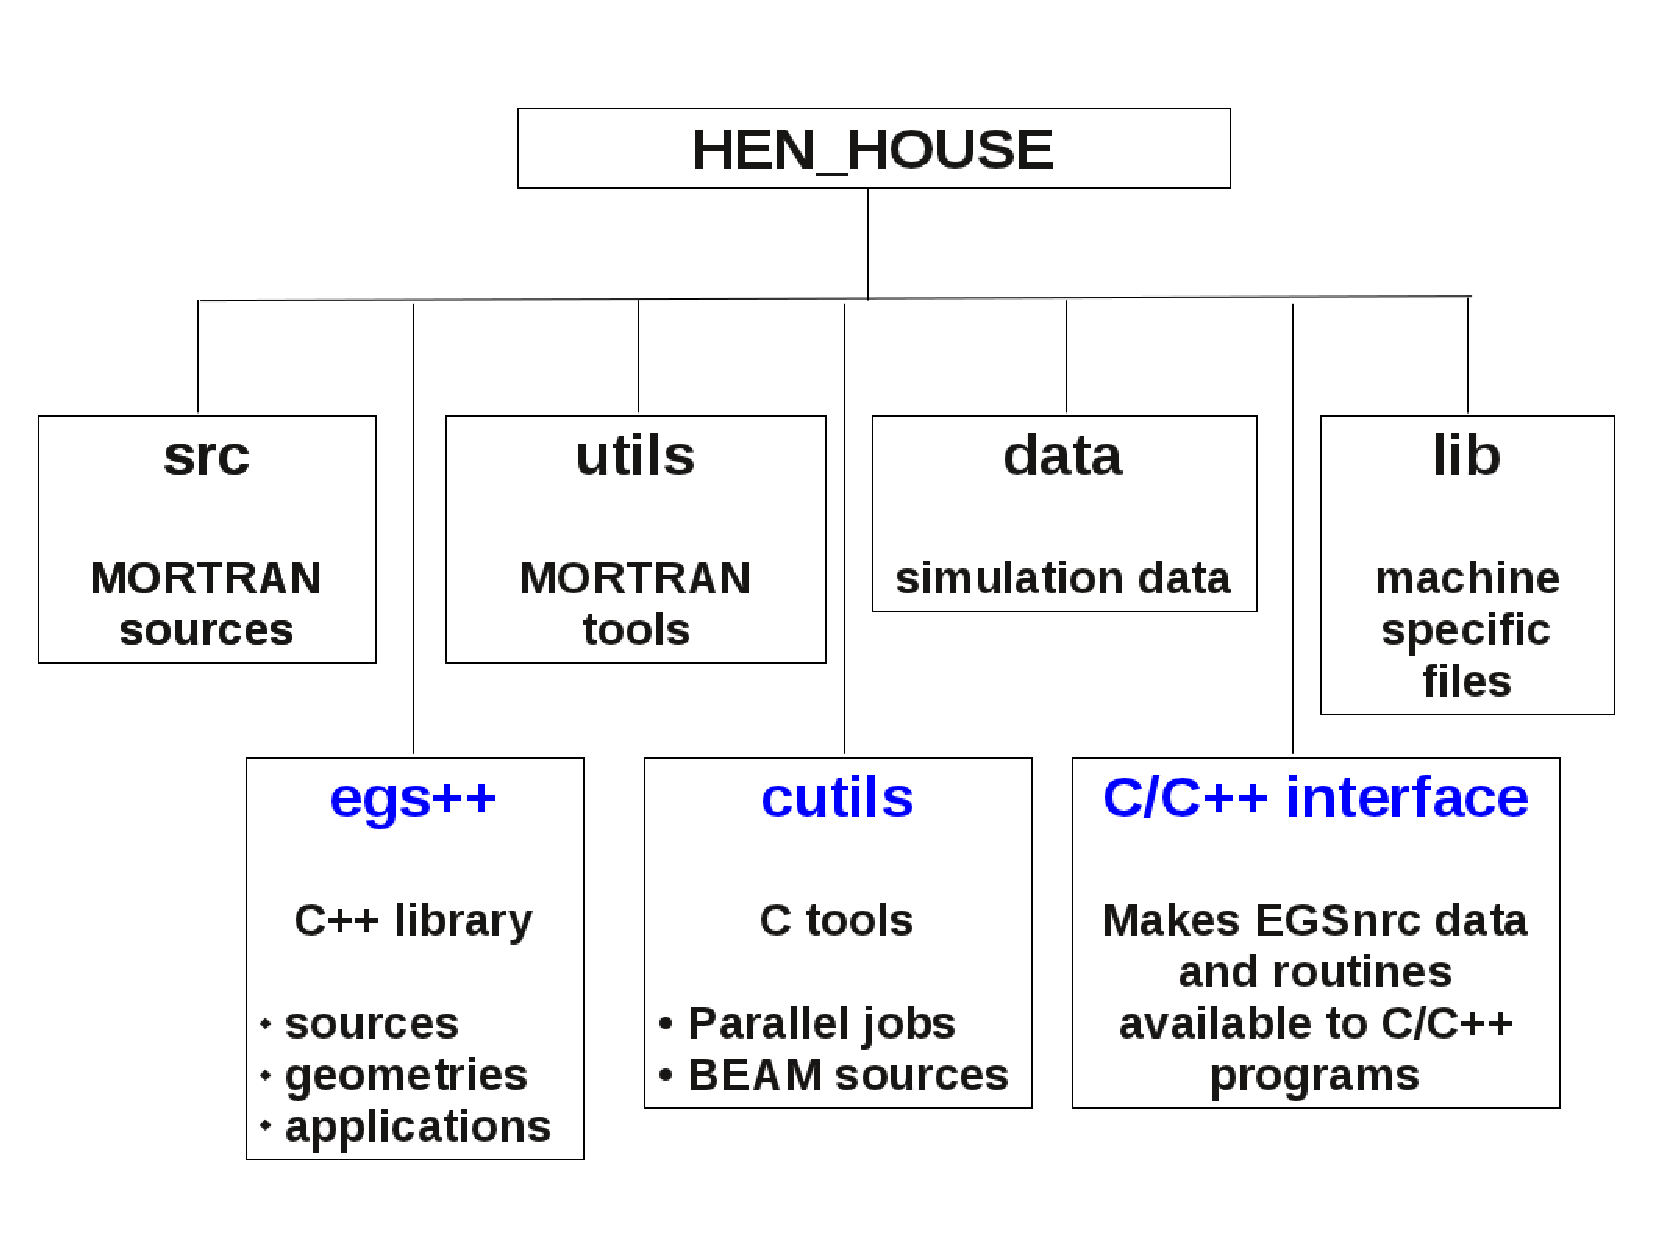
\includegraphics[width=5.5in]{figures/egs_file_structure_with_egspp}
\end{center}

To compile EGSnrc on linux, there is a command line script that can be used instead of the installation GUI:

\Verb+$HEN_HOUSE/scripts/configure+

This script does not create the \Verb+$EGS_HOME+ directory! Run the finalize script to create \Verb+$EGS_HOME+, copy over application source and compile applications. At the end of this script, the suggested environment variables are printed as output to the terminal:

\Verb+$HEN_HOUSE/scripts/finalize_egs_foruser+

It is possible to have EGSnrc configured for execution on several servers. This means that the configuration script is run once on each machine, set to use a different machine name each time. On each server, the \Verb+$EGS_CONFIG+ environment variable must be set uniquely, and should point to the main configuration file created by the installation script (but type it in as an absolute path, don't use environment variables):

\Verb+$HEN_HOUSE/specs/$my_machine.conf+

On linux systems, the \Verb+$HEN_HOUSE+ and \Verb+$my_machine+ environment variables are actually extracted and automatically set \textit{using} the \Verb+$EGS_CONFIG+ environment variable that you provide.

\subsection{The \$EGS\_HOME}
The \Verb+$EGS_HOME+ directory contains all of the applications and data created or provided by the user. Each application (previously called a \Verb+user_code+) has its own directory which contains the source code, a Makefile, and the user's input files. Output files from simulations are also produced in the application directories.

The user may store their own set of material data in \Verb+$EGS_HOME/pegs4+, which will automatically supplement the data that is available in \Verb+$HEN_HOUSE/pegs4+.

\Verb+BEAMnrc+ has a folder structure different from other applications. Each accelerator that is built for \Verb+BEAMnrc+ is assigned its own directory with the name \Verb+BEAM_yourAccel+, where \Verb+yourAccel+ is the name of the accelerator. In other words, each accelerator is compiled as an independent EGSnrc application. The component module specifications for all accelerators are contained in \Verb+$EGS_HOME/beamnrc/spec_modules+.

The compiled executables for applications reside in \Verb+$EGS_HOME/bin/$my_machine+.

\begin{center}
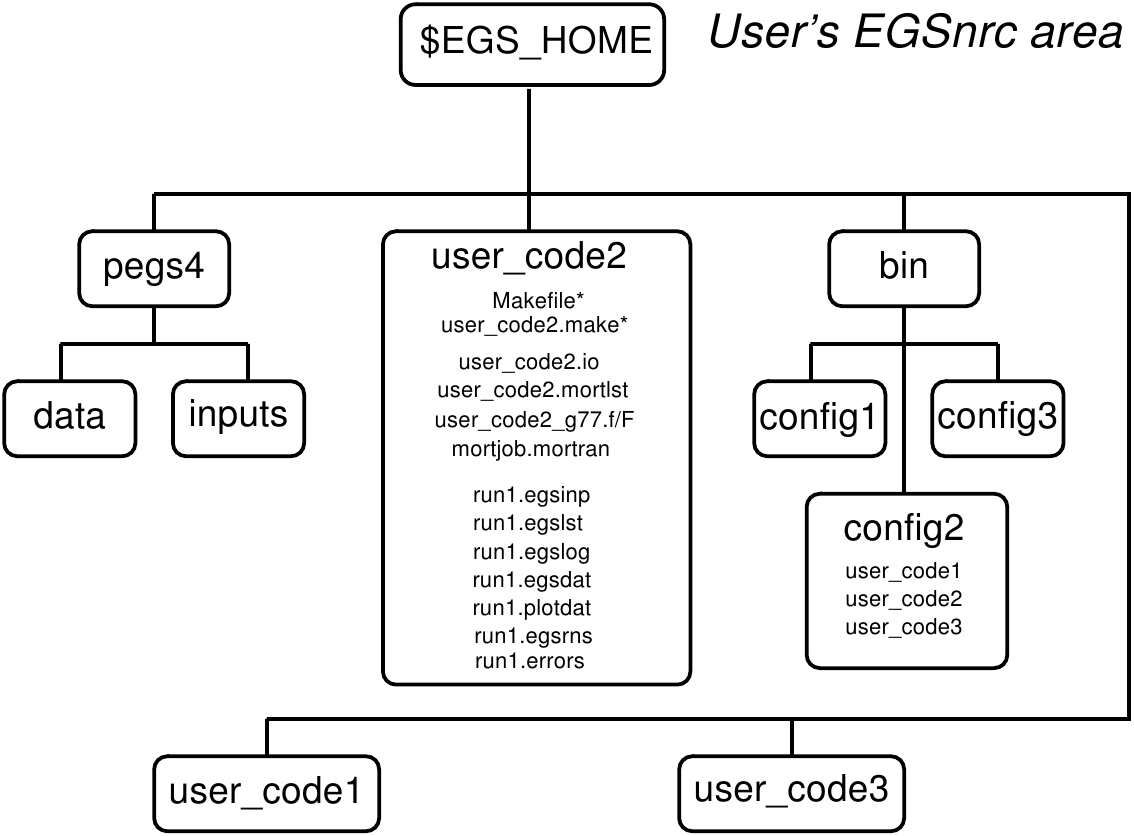
\includegraphics[width=5in]{figures/Users_EGSnrc_area}
\end{center}



% \section{References}
% \renewcommand{\rightmark}{References}
% \vspace*{-1cm}
% \setlength{\baselineskip}{0.5cm}
% \bibliography{../irs}
% \bibliographystyle{unsrt}

\end{document}
